\section{Geometry-based shading Approach}
The key of this approach is  \textit{incorporating surface curvature} information into shape depiction enhancement technique. This is done with multiple steps:
\begin{enumerate}
	\item  \textbf{3D Shape Descriptor:} 3D Object surface shape is analyzed using the shape descriptor. \textbf{Curvature computation} extracts salient surface features. The contribution can be controlled using some parameters.
	\item \textbf{Geometry-based Shading:} Surface normals are \textit{smoothed} or \textit{sharpened} to attenuate or exaggerate the surface depiction; Then, the \textbf{reflected lightning intensity} is scaled using also surface curvature previously calculated.
	\item \textbf{Rendering:} This shading technique is applied to various \textbf{non-photorealistic rendering styles}, reformulating the reflected radiance equation in a way that takes the enhanced shading into account.
\end{enumerate}
In \textbf{Figure \ref{fig:method}} the rendering pipeline is graphically illustrated.
\begin{figure}[h]
	\centering
	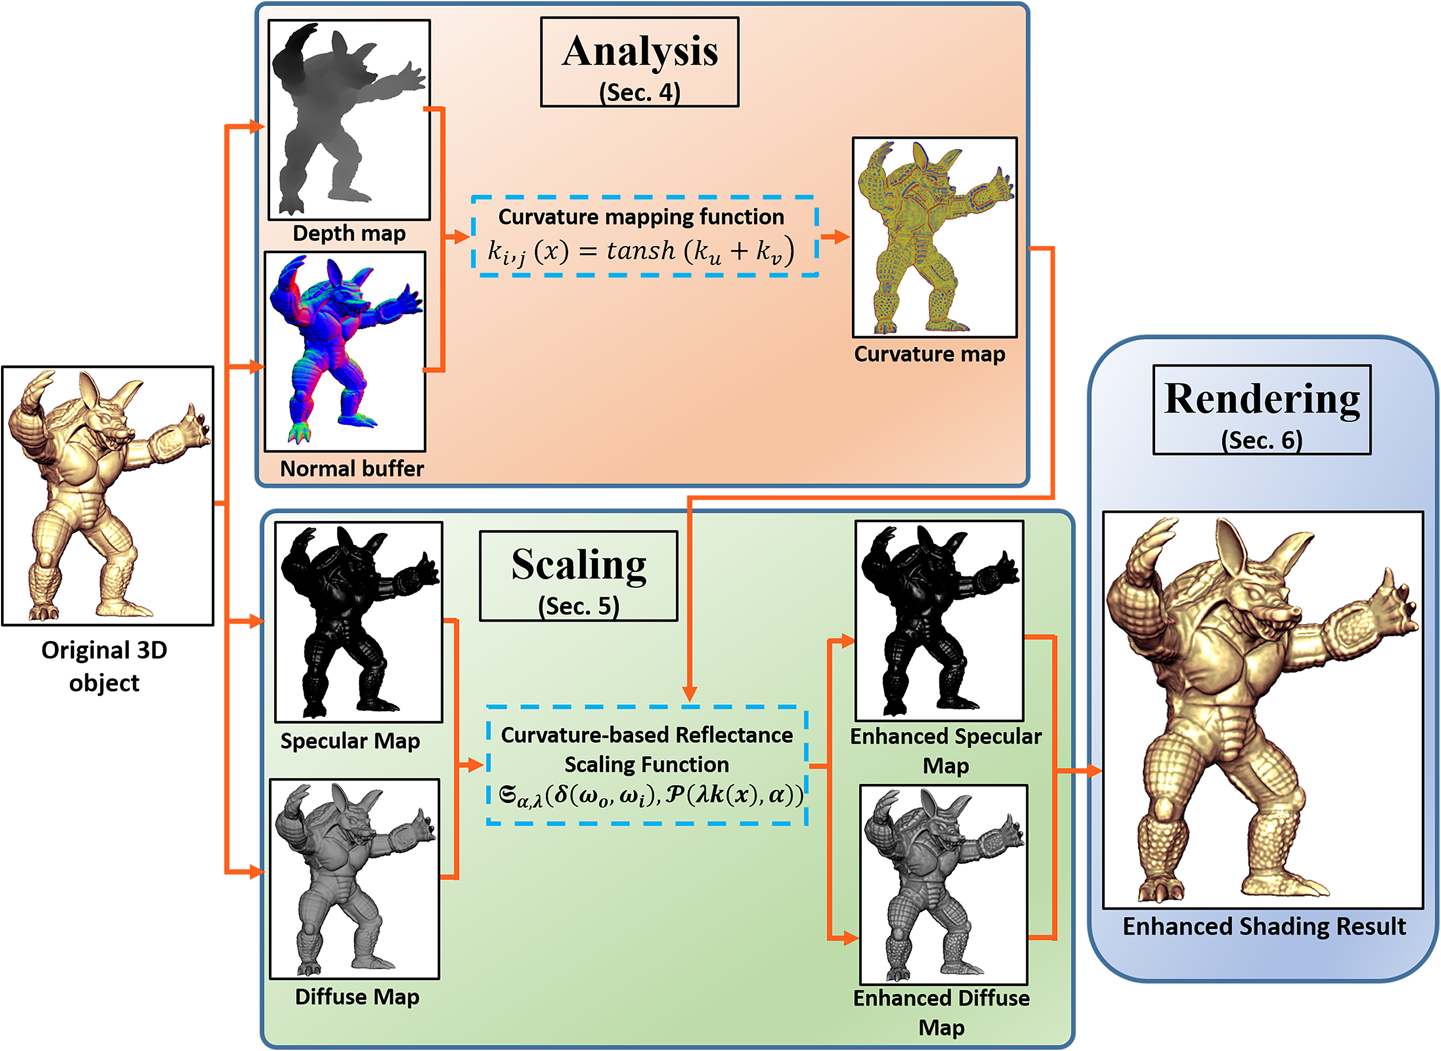
\includegraphics[width=0.75\textwidth]{Images/method.png}
	\caption{The rendering pipeline of the paper's approach. It combines estimating the surface curvature, scaling the reflected lighting and rendering the NPR result}
	\label{fig:method}
\end{figure}